\documentclass[../main/main.tex]{subfiles}

\newdate{date}{6}{12}{2019}


\begin{document}

\section{First-order phase transitions in Landau theory}
\marginpar{ \textbf{Lecture 16.} \\  \displaydate{date}. \\ Compiled:  \today.}

As we have seen, Landau theory is based on the assumption that the order parameter is small near the critical point, and we have seen in the example of the Ising model how it can describe a continuous phase transition (in fact, for \( t \rightarrow 0 \) we have \( \eta \rightarrow 0 \)).
However, because of the symmetry properties of the Ising model we have excluded any possible cubic term; what we now want to do is to consider a more general form of
\( \mathcal{L} \) which includes also a cubic term in \( \eta  \) (in the case in which the symmetry is not violated), and see that this leads to the occurrence of a first-order phase transition.
In fact, we want to generalize to include multicritical points, or phase transitions. Let us remember that in the Ising model we have phase transition derived by symmetry breaking, while now we have another type of phase transitions.

We have seen that since the order parameter is null for \( T > \bar{T}  \) the Landau free energy cannot contain any linear term in \( \eta  \). Let us therefore consider the simplest Landau free energy that depends on a particular field:
\begin{empheq}[box=\myyellowbox]{equation}
\mathcal{L} ( \eta ,t,h)= a t \eta ^2 - w \eta ^3 + \frac{b}{4} \eta ^4 - h \eta
\label{eq:16_5}
\end{empheq}
where \( t \equiv \frac{T-T^*}{2} \) and \( w \) is an additional parameter that we fix to be positive, \( w>0 \); as in the previous case, we must have \( b>0 \) so that \( \eta  \) has finite values in the equilibrium configurations. In addiction,
\begin{equation*}
  a t = \frac{a}{2} ( T - T^*) \quad \begin{cases}
    > 0 & \text{ if } T > T^* \\
    <0 & \text{ if } T < T^*
\end{cases}
\end{equation*}
\begin{remark}
For \( w<0 \) the results are the same, but in the \( \eta <0 \) diagram.
\end{remark}
The temperature \( T^* \) is the one at which we have the continuous transition if \( w=0 \), but as we will see it doesn't have great significance now. The equilibrium configurations of the system,  will be given by:
\begin{equation*}
  \pdv{\mathcal{L}_G}{\eta } = 0 \quad \Rightarrow h = 2 a t \eta - 3 w \eta ^2 + b \eta ^3
\end{equation*}
In absence of external fields (\( h=0 \)), the equilibrium states becomes
\begin{equation*}
  h = 0 \quad \Rightarrow \eta ( 2 a t - 3 w \eta  + b \eta ^2) = 0
\end{equation*}
The solutions of this equation are
\begin{equation}
  \begin{cases}
   \bar{\eta } = 0 & \text{disordered phase}\\
  \bar{\eta_\pm } = \frac{1}{2b} \qty(3w \pm \sqrt{9 w^2 - 8abt} ) & \text{ordered phases}
  \end{cases}
\end{equation}
Let us rewrite the ordered solutions as
\begin{equation}
  \bar{\eta }_{\pm} = \frac{1}{2b} \qty(3w \pm \sqrt{9 w^2 - 8abt} ) = c \pm \sqrt{c^2 - \frac{2at}{b}}
  \label{eq:16_3}
\end{equation}
with
\begin{equation*}
  c = \frac{3w}{2b}
\end{equation*}
However, these two last solutions are possible only if:
\begin{equation*}
  \bar{\eta }_{\pm} \in \R \iff c^2 - \frac{2at}{b}>0  \iff t = \frac{T-T^*}{2} < \frac{c^2 b}{2a} \equiv t^{**} \equiv  \frac{T^{**}-T^*}{2}
\end{equation*}
Hence, we have
\begin{equation*}
  T^{**} = T^* + \frac{c^2b}{a} = T^* + 2t^{**}
\end{equation*}
so, since \( t^{**} \) is positive, this will occur at temperatures higher than \( T^* \).
Let us consider different cases:
\begin{itemize}
\item If \( t> t^{**} \) \( ( T > T^ {**}) \), then the system will be in the disordered phase and we have  \( \bar{\eta }_\pm \notin \R  \). The only real solution is \( \bar{\eta }=0  \) that is also the absolute minimum of \( \mathcal{L} \). The plot is shown in Figure \ref{fig:16_1}.
\begin{figure}[h!]
\centering
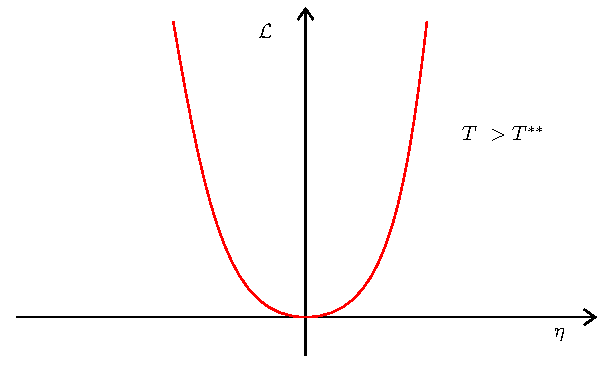
\includegraphics[width=0.6\textwidth]{../lessons/16_image/1.pdf}
\caption{\label{fig:16_1} Landau free energy for \( t> t^{**} \) \( ( T > T^ {**}) \). The point \( \bar{\eta }=0  \) is the absolute minimum.}
\end{figure}


\item If \( t \le t^{**} \) \( ( T \le T^ {**}) \), we have \( \bar{\eta }_\pm = c \pm \sqrt{c^2 - \frac{at}{b}} \in \R  \) are both possible solutions. One will be a local maximum and the other a local minimum.

  \begin{itemize}
  \item At \( T = T^{**}\), we have \( \bar{\eta }_- = \bar{\eta }_+   \) (flex point), as shown in Figure \ref{fig:16_2}.
  \begin{figure}[h!]
  \centering
  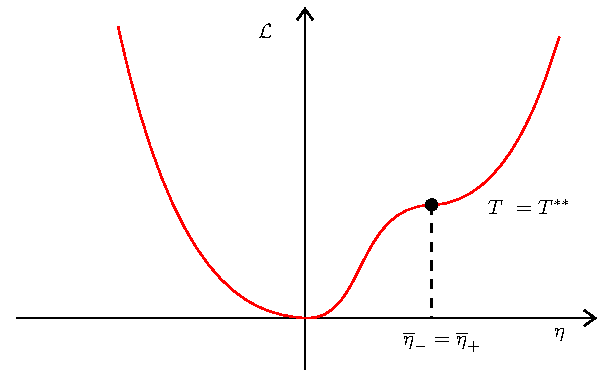
\includegraphics[width=0.6\textwidth]{../lessons/16_image/2.pdf}
  \caption{\label{fig:16_2} Landau free energy for \( t\le t^{**} \) \( ( T = T^ {**}) \). The point \( \bar{\eta }_- =\bar{\eta }_+   \) is a flex one.}
  \end{figure}


  \item For \( T_t < T < T^{**} \), a new minimum appears at \( \eta = \bar{\eta }_+   \), but we will have \( \mathcal{L} (\bar{\eta }_+) >0  \), so  this is only a local minimum (since \( \mathcal{L}(0)=0 \)):  in this range of temperatures the ordered phase is metastable. The plot is shown in Figure  \ref{fig:16_3}.
  \begin{figure}[h!]
  \centering
  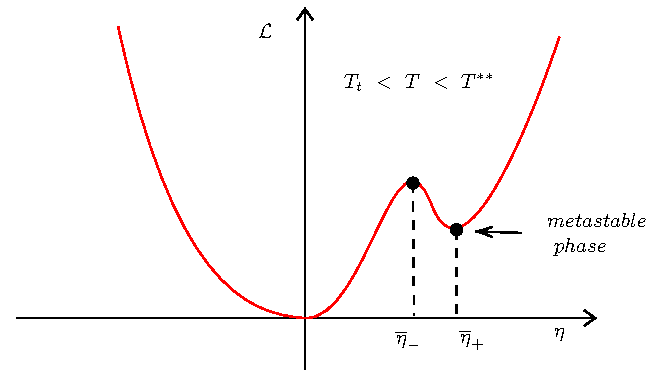
\includegraphics[width=0.6\textwidth]{../lessons/16_image/3.pdf}
  \caption{\label{fig:16_3} Landau free energy for \( t\le t^{**} \) \( ( T_t <T \le T^ {**}) \). The point \( \bar{\eta }_+   \) is a local minimum.}
  \end{figure}


  \item If we further decrease the temperature \( T \), we will reach a temperature \( T=T_t \) for which \(\mathcal{L} (\bar{\eta }_+ ) = 0 = \mathcal{L}(0)  \):  at this point the ordered and disordered phase coexist, so this is the temperature of a new transition! The plot is shown in Figure  \ref{fig:16_4}. \( T_t \)  is given by the coexistence condition
  \begin{equation*}
    \mathcal{L} (\bar{\eta }_+ ) = \mathcal{L} (0)
  \end{equation*}
  that is the coexistence between the disordered and ordered phases. In fact, in the plot of Figure \ref{fig:16_4} we see that there are two minima in the same line, this is  a first order transition.

  \begin{figure}[h!]
  \centering
  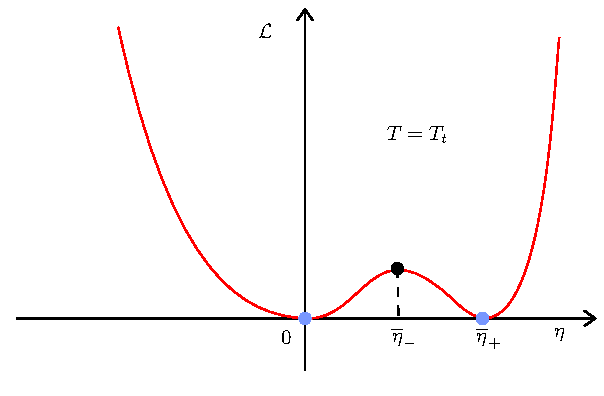
\includegraphics[width=0.6\textwidth]{../lessons/16_image/4.pdf}
  \caption{\label{fig:16_4} Landau free energy for \( t\le t^{**} \) \( ( T = T_t ) \). The point \( \bar{\eta }_+   \) is a minimum. The ordered and disordered phase coexist.}
  \end{figure}


  \item Finally for \( T^* < T < T_t \), \( \mathcal{\bar{\eta }_+ } \) becomes negative and so now \( \eta = \bar{\eta }_+  \) is the global minimum of \( \mathcal{L} \):  the ordered phase becomes stable and the disordered phase metastable, indeed now \( \eta =0 \) is only a local minimum (see Figure \ref{fig:16_5}).

  \begin{figure}[h!]
  \centering
  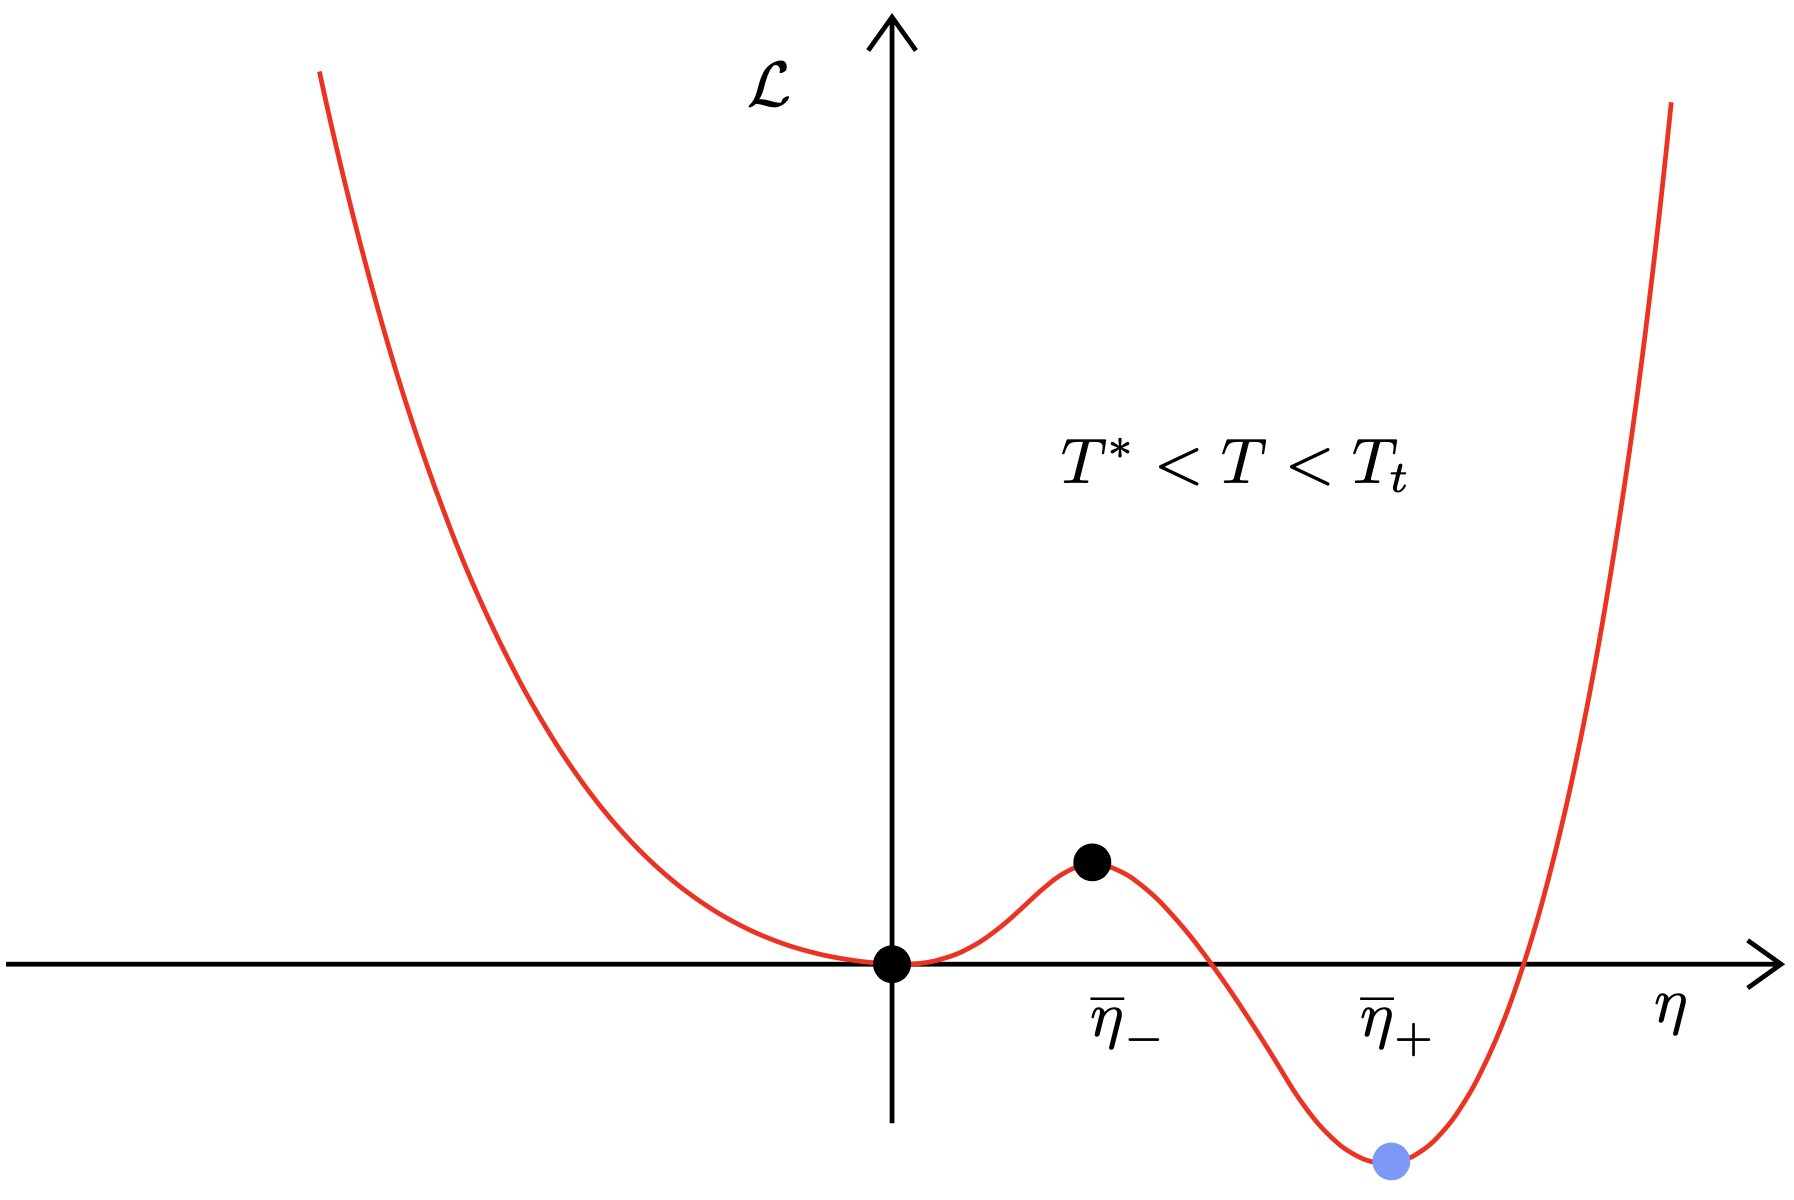
\includegraphics[width=0.6\textwidth]{../lessons/16_image/5.jpg}
  \caption{\label{fig:16_5} Landau free energy for \( t\le t^{**} \) \( ( T^*< T <T_t ) \). The point \( \bar{\eta }_+   \) is the global minimum.}
  \end{figure}


  \item  If now \( T < T^*\), \( \mathcal{L} \) develops a new minimum for \( \eta <0 \), but it is only a local minimum (the asymmetry introduced by \( -w \eta ^3 \) ensures that \( \bar{\eta }_+  \) is always the global minimum).
  This means that also for \( T< T^* \)  the disordered phase with \( \bar{\eta }_+  \) continues to be the stable one, and so no phase transition occurs at \( T^* \)  any more; this is what we meant when we said that \( T^* \) is not a relevant temperature any more.
  \end{itemize}

  \begin{figure}[h!]
  \begin{minipage}[c]{0.55\linewidth}
  \subfloat[][First-order transition.]{ 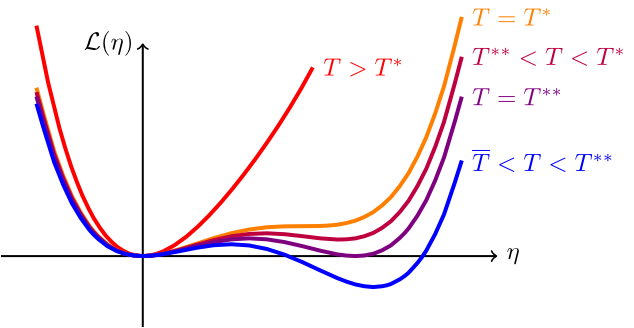
\includegraphics[width=0.8\textwidth]{../lessons/16_image/p_1.png}  \label{fig:} }
  \end{minipage}
  \begin{minipage}[]{0.55\linewidth}
  \centering
  \subfloat[][Same transition for lower values of the temperature.]{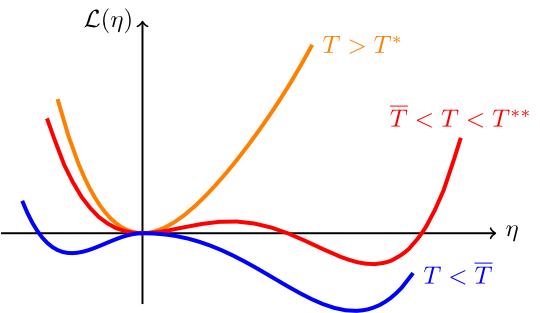
\includegraphics[width=0.8\textwidth]{../lessons/16_image/p_2.png}  \label{fig:} }
  \end{minipage}
  \caption{\label{fig:16_p} The notation in this plot is different from the one used previously. Here \( \bar{T} \equiv T^*  \), \( T^{*} \equiv T^{**} \) and \( T^{**} \equiv T_t \).  }
  \end{figure}

Therefore, we have seen that lowering the temperature of the system, the value of \( \eta  \) for which \( \mathcal{L} \) has a global minimum changes discontinuously from \( \eta =0 \)  to \( \bar{\eta }_+  \): this is a first-order transition. All the results obtained are shown in Figure \ref{fig:16_p}.

\end{itemize}


  As we said, at \( T=T_t \) the system undergoes a first order transition. It is defined by two conditions: it must be a minimum of \( \mathcal{L} \) and such that the value of \( \mathcal{L} \) in that minimum is zero.  Thus we can determine \( T_t \) as follows:
  \begin{equation*}
    \begin{cases}
     \pdv{\mathcal{L}}{\eta } = 0 = \eta \qty(2 a t - 3 w \eta +  b \eta ^2)  & \text{extreme condition}\\
    \mathcal{L} ( 0 ) = \mathcal{L} ( \eta _+)=0 = \eta ^2 (a t - w \eta + \frac{b}{4} \eta ^2)& \text{coexistence condition}
    \end{cases}
  \end{equation*}
  Therefore, for \( \eta \neq 0 \):
  \begin{equation*}
  \Rightarrow
    \begin{cases}
     2 a t - 3 w \eta +  b \eta ^2 = 0\\
     a t - w \eta + \frac{b}{4} \eta ^2 = 0
    \end{cases}
  \end{equation*}
  Solving with respect to \( \eta  \)  and \( t \), we get
  \begin{equation*}
    \begin{cases}
     \bar{\eta }_{t} = + \frac{2w}{b} >0 \\
      t_t = \frac{2w^2}{ab}
    \end{cases}
  \end{equation*}
Since by the definition \( t = (T-T^*)/2 \), we have:
  \begin{equation}
    T_t = T^* + \frac{4w^2}{ab}
    \label{eq:16_6}
  \end{equation}
  \begin{remark}
  Let us note that \( T_t >T^* \).
  \end{remark}
  Since at \( T= T_t \) there is a first order transition does the system display latent heat?
  \begin{equation*}
    s = \eval{- \pdv{\mathcal{L}}{T} }_{\eta _t} = - \frac{1}{2} a \bar{\eta }_t^2 = - \frac{a}{2} \qty(\frac{2w}{b})^2
  \end{equation*}
  Hence, there is an entropy jump.
  The latent heat absorbed to go from the ordered to the disordered phase is
  \begin{equation}
    q = - T_t s = \frac{a}{2} T_t \qty(\frac{2w}{b})^2
  \end{equation}




\subsection{Phase stability and behaviour of \( \pmb{\chi _T }\)}
Finally, we can also determine the susceptibility of the system:
\begin{equation*}
  \chi _T \equiv \pdv{\eta }{h}
\end{equation*}
In the presence of an external field, let us derive the equation of state with respect to \( h \):
\begin{equation*}
  \pdv{}{h} \qty(\pdv{\mathcal{L}_G}{\eta } = 0 )   = \pdv{}{h} \qty(2 a t \eta - 3 w \eta ^2 +  b \eta ^3 = h)
\end{equation*}
Hence, since \(   \chi _T \equiv \pdv{\eta }{h} \),
\begin{equation*}
   \chi \qty(2 a t - 6 w \eta + 3 b \eta ^2 ) =1
\end{equation*}
The result is
\begin{equation}
  \chi _T = \frac{1}{2 a t - 6 w \eta + 3 b \eta ^2}
  \label{eq:16_1}
\end{equation}
We now make use of equation \eqref{eq:16_1} to compute the limit of stability of the phases we have found.

\subsection{Computation of \( T^{**} \) }
As said, \( T=T^{**} \) is the value below which the ordered phase becomes a metastable state (local minima). In particular, since for \( T=T^{**} \) the point \( \bar{\eta }_-=  \bar{\eta }_+ \) is a flex point, we have the condition
\begin{equation*}
    \pdv[2]{\mathcal{L}}{\eta } = 0
\end{equation*}
thus:
\begin{equation*}
    \pdv{}{\eta } \qty(   2 a t \eta  - 6 w \eta^2 + b \eta ^3 = h ) = 0 \quad  \Rightarrow   2 a t - 6 w \eta + 3b \eta ^2 = \pdv{h}{\eta } =  \chi ^{-1} = 0
\end{equation*}
Remember that at \( T=T^{**} \)  the two solutions \( \bar{\eta }_\pm \) coincide, hence from Eq.\eqref{eq:16_3} we have
\begin{equation*}
  c^2 - \frac{2at}{b} = 0 \quad \Rightarrow \bar{\eta }_\pm = \eta _2 = \frac{3 w}{2 b}
\end{equation*}
Inserting in the expression with \( \chi ^{-1} =0 \), we have
\begin{equation*}
  \chi ^{-1} = 0 = 2 a t^{**} - 6 w \bar{\eta }_2 + 3 b \bar{\eta }_2^2
\end{equation*}
Hence,
\begin{equation}
  \iff t^{**} = \frac{9 w^2}{8 a b} = \frac{1}{2} \qty(T^{**}-T^*)
\end{equation}
Remind that for \( T_t < T < T^{**} \) the ordered phase \( \bar{\eta }_+  \) is metastable.


\subsection{Computation of \( T^* \)}
The instability of the disordered phase \( \eta =0 \) is when \( \mathcal{L} \) presents a flex point at \( \eta =0 \). Therefore, from the condition
\begin{equation*}
    \eval{\pdv[2]{\mathcal{L}}{\eta }}_{\bar{\eta } = 0 } = 0
\end{equation*}
we have
\begin{equation*}
  \chi ^{-1} = 2 a t - 6 w \eta + 3b \eta ^2 = \pdv{h}{\eta } = 0 \quad \Rightarrow
  2 a t = 0 \Rightarrow t=0
\end{equation*}
Hence, we have
\begin{equation}
\Rightarrow T = T^*
\end{equation}
thus no phase transition occurs at \( T^* \) any more. The plot of the Landau free energy in the case \( T=T^* \) is shown in Figure \ref{fig:16_6}.

\begin{figure}[h!]
\centering
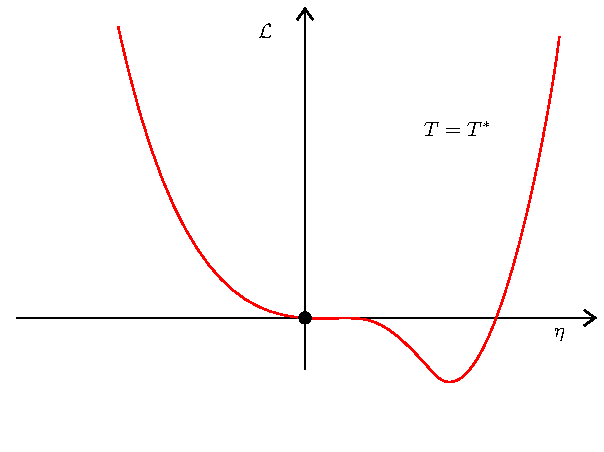
\includegraphics[width=0.6\textwidth]{../lessons/16_image/6.pdf}
\caption{\label{fig:16_6} Landau free energy for \( t\le t^{**} \) \( ( T =T^* ) \). The point \( \bar{\eta }_+   \) is the global minimum, while the point \( \bar{\eta }  = 0  \) is a flex point.}
\end{figure}





\section{Multicritical points in Landau theory}
It is possible for a system to have more "disarranging parameters" than the only temperature \( T \); let us call one such field \( \Delta  \). In this case the phase diagram of the system becomes richer, with coexistence and critical lines that intersect in points called multicritical points; one of the most common examples of a multicritical point is the \emph{tricritical point}, which divides a first-order transition line from a second-order one. An example of a system of the type we are considering is the Blume-Emery-Griffiths model, which we have studied in Mean field theory for the Blume-Emery-Griffiths model. In that case the additional "disarranging field" was the concentration \( x \)  of \( \text{He}^3 \), and the tricritical point is the one we called \( (x_t,T_t) \).

Such a phenomenology can be obtained within Landau theory also with terms different from a simple cubic one; in particular, we can have first order phase transitions even when the system is invariant under parity, like in the case of the Ising model. In fact in that situation we required the coefficient of \( \eta ^4 \) to be always positive, but if this is not true then \( \mathcal{L} \) will be:
\begin{equation}
  \mathcal{L} (T, \Delta, \eta ) = \frac{a (t,\Delta )}{2} \eta ^2 + \frac{b(t,\Delta )}{4} \eta ^4 + \frac{c}{6} \eta ^6 - h \eta
\end{equation}
where \( a,b \) and \( c \) are functions of two parameteres \( (T,\Delta ) \) and \( c>0 \) positive for the stability of the system (otherwise, like in the case previously considered, the minimization of \( \mathcal{L} \) leads \( \eta  \) to infinity); \( \Delta  \) is the disordered field (in the BEG model \( \Delta  \) was the \( \% \, \text{He}^3\) atoms).

\begin{remark}
To allow the coefficient of \( \eta ^4 \) to change sign, we need the \( \eta ^6 \) term.
\end{remark}



Let us study the phenomenology of \( \Delta  \) (\( \Delta _c \) is a critical value):

\begin{itemize}

\item If \( \Delta < \Delta _c \): as \( T \) decreases, \( a(T,\Delta ) \) decreases and, at \( T = T_c (\Delta ) \), becomes zero. In this region \( b(T,\Delta ) >0 \) and the system displays the standard \( (\eta ^4) \) critical point. At \( T= T_c \) we have:
\begin{equation*}
  T = T_c (\Delta ) \Rightarrow \begin{cases}
    a (T_c,\Delta ) = 0 \\
    b (T_c,\Delta ) > 0
\end{cases}
\end{equation*}

If \( a \) changes sign and  \( b \) is kept positive (which can be done varying the values of \( T \) and \( \Delta  \) in a way such that \( a \) goes to zero faster than \( b \), depending of course on their explicit expressions) then a critical transition occurs since in this case \( \eta =0 \)  becomes a local maximum for \( \mathcal{L} \), and it develops two new global minima. Therefore, the solution of the equation  \( a(T,\Delta )=0 \)  will give a line of critical points in  \( (T,\Delta ) \) plane.

\item If \( \Delta > \Delta _c \): as \( T \) decreases, \( b(T,\Delta ) \) becomes zero before \( a(T,\Delta ) \). At \( T=T_c \) we have
\begin{equation*}
    T = T_c (\Delta ) \Rightarrow \begin{cases}
    a (T_c,\Delta ) > 0 \\
    b (T_c,\Delta ) = 0
\end{cases}
\end{equation*}
Hence, if \( b \) becomes negative while \( a \) is still positive (which again can be done varying \( T \) and \( \Delta  \) so that \( b \) vanishes faster than \( a \)) then something rather different happens: in this case, one can show that as  \( b \) approaches zero \( \mathcal{L} \)  develops two new symmetric local minima at \( \bar{\eta }_\pm  \) (similarly to the case analysed before, with the difference that now the situation is perfectly symmetric since \( \mathcal{L} \) is even) and they will become the new global minima as \( \mathcal{L} (\bar{\eta }_\pm ) = 0 \),
 which happens when \( b \) changes sign: this way the equilibrium value of the order parameter change discontinuously from zero to a non-zero quantity so a first-order transition has indeed happened.

In this case, we have
\begin{equation*}
 \mathcal{L} = a \eta ^2 + c \eta ^6, \quad a>0
\end{equation*}
The equilibrium states are
\begin{equation*}
  \pdv{\mathcal{L}}{\eta } = 2 a \eta + 6 c \eta ^5 = 0
\end{equation*}
so, the solutions are
\begin{equation*}
   \begin{cases}
    \eta =0 \\
    \eta _{1,2,3,4}
  \end{cases}
\end{equation*}


\begin{figure}[h!]
\centering
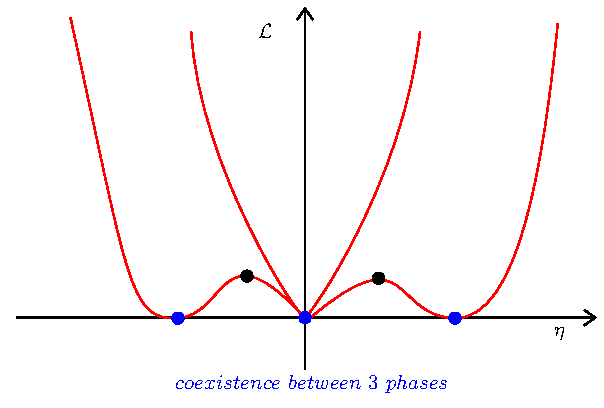
\includegraphics[width=0.6\textwidth]{../lessons/16_image/7.pdf}
\caption{\label{fig:16_7} Landau free energy for \( \Delta > \Delta _c \). There is coexistence between three phases, in fact there are 3 global minima.}
\end{figure}




\item Case \( \Delta = \Delta _t  \): the tricritical point is given by the values of \( \Delta = \Delta _t \)  and \( T= T_c \) such that
\begin{equation*}
  a (\Delta _t, T_t) = b (\Delta _t, T_t) = 0
\end{equation*}
 This means that when both \( a \) and \( b \) are null the system goes from exhibiting a continuous critical transition to a discontinuous first-order one; in other words, the tricritical point \( (T_{c},\Delta _{c}) \)  can be determined from the solution of the equations \( a(T,\Delta )=0 \) and \(b(T,\Delta )=0  \).

At the tricritical point the system is described by the following Landau free-energy:
\begin{equation*}
  \mathcal{L}_t = c \eta ^6 - h \eta
\end{equation*}
The equation of state is
\begin{equation*}
  \pdv{\mathcal{L}_t}{\eta } = 0 \quad \Rightarrow  h = 6 c \eta ^5
\end{equation*}

\end{itemize}

\noindent The first-order transition with an even \( \mathcal{L} \) are shown in Figure \ref{fig:16_f}.

\begin{figure}[h!]
\centering
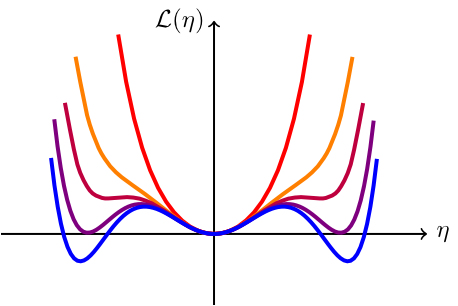
\includegraphics[width=0.6\textwidth]{../lessons/16_image/f.png}
\caption{\label{fig:16_f} First-order transition with an even \( \mathcal{L} \).}
\end{figure}


To conclude let us consider again a system with an Ising-like Landau free energy, where \( c>0 \) and  \( a,b \)  are in general functions of the reduced temperature \( t \)  (and also of the other "disarranging" parameter \( \Delta  \), which we now neglect). The Landau free energy is again
\begin{equation*}
  \mathcal{L}  = \frac{a }{2} \eta ^2 + \frac{b}{4} \eta ^4 + \frac{c}{6} \eta ^6 - h \eta
\end{equation*}

 We now want to show that we can understand how the phase diagram of the system is in  \( (a,b) \) space, i.e. that we can draw where the phase transition lines are and so we are able to visually represents where the various phases of the system are in \( (a,b) \) plane.

 First of all, we can note that when \( a,b>0 \) the only minimum of \( \mathcal{L} \)  is  \( \bar{\eta }=0  \), so the system is in the paramagnetic phase. Furthermore if \( a<0 \)  and  \( b>0 \) the system is in the magnetic phase, and a second order transition has occurred; therefore we can surely say that the half-line  \( a=0,b>0 \) is a second order transition line.

 We must thus determine where the first order transition line lies in \( (a,b) \) space. In order to do so, we first note that the extrema of \( \mathcal{L} \)  are given by:
\begin{equation*}
 0={\frac {\partial {\mathcal {L}}}{\partial \eta }}=\eta (a+b\eta ^{2}+c\eta ^{4})\quad \Rightarrow \quad {\bar {\eta }}_{\pm }^{2}={\frac {-b\pm {\sqrt {b^{2}-4ac}}}{2c}}
\end{equation*}
(and of course they exist only when the temperature is such that \( b^{2}-4ac>0 \)) and since:
\begin{equation*}
  \displaystyle {\frac {\partial ^{2}{\mathcal {L}}}{\partial \eta ^{2}}}_{|{\overline {\eta }}_{\pm }}=\pm {\overline {\eta }}_{\pm }^{2}\cdot 2{\sqrt {b^{2}-4ac}}
\end{equation*}
we have that \( \pm \bar{\eta }_+  \) are maxima while \( \pm \bar{\eta }_-  \) are minima. The first order transition happens when \( \mathcal{L} (\pm \bar{\eta }_\pm  )  = \mathcal{L} (0) = 0 \), so:
\begin{equation*}
{\frac {a}{2}}{\bar {\eta }}_{+}^{2}+{\frac {b}{4}}{\bar {\eta }}_{+}^{4}+{\frac {c}{6}}{\bar {\eta }}_{+}^{6}=0\quad \Rightarrow \quad {\frac {a}{2}}+{\frac {b}{4}}{\bar {\eta }}_{+}^{2}+{\frac {c}{6}}{\bar {\eta }}_{+}^{4}=0
\end{equation*}
Now, from the condition  \(\partial {\mathcal {L}}/\partial \eta =0  \) we can express \( \bar{\eta }_{+}^{4}  \) as a function of \( \bar{\eta }_{+}^{2}  \), and we get \( \bar {\eta }_{+}^{4} =- (a+b \bar {\eta }_{+}^{2})/c \).
 Substituting we get:
\begin{equation*}
   \bar {\eta }_{+}^{2}=-4\frac {a}{b}
\end{equation*}
and substituting again in \( \bar {\eta }_{+}^{2} =(-b+\sqrt {b^2-4ac} )/(2c) \)  in the end we get:
\begin{equation*}
  b=-4 \sqrt { \frac {ac}{3} }
\end{equation*}
so the first order transition line is a parabola in \( (a,b) \)  plane (in particular it will lie in the fourth quadrant). In the end the situation is as in Figure \ref{fig:16_8}. As we can see the tricritical point of the system, being the point that divides the first-order from the second-order transition line, is the origin \( (0,0) \) of the parameter space.

\begin{figure}[h!]
\centering
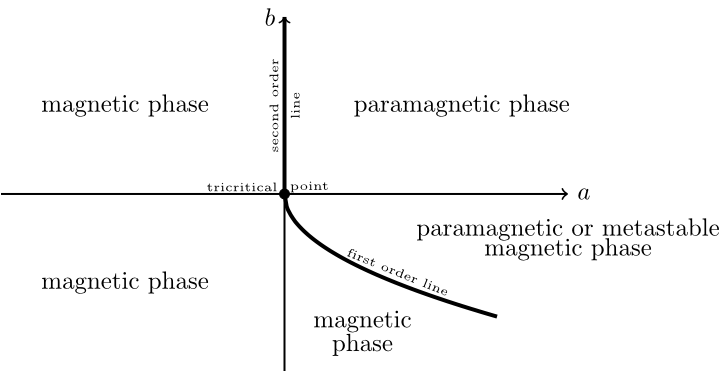
\includegraphics[width=0.8\textwidth]{../lessons/16_image/8.png}
\caption{\label{fig:16_8} Phase diagram of the system in  \( (a,b) \) space.}
\end{figure}




\section{Liquid crystals}
We now proceed to study a particular physical system, liquid crystals, to which we will apply Landau theory of phase transitions. As we will see the symmetries of the system will allow the Landau free energy to include a cubic term in the order parameter (which we will properly define), and so we will be able to describe the first-order transition from an isotropic to a nematic phase (which we are now going to introduce).

\subsection{What are liquid crystals?}
Liquid crystals phase (LC) can be seen as an intermediate phase between a liquid and a solid: they are liquid like any other conventional fluid, but also have internal orientetional order like solid crystals. This orientational order provides them particular anisotropic properties from an optical, electric and magnetic point of view. The most common structural characteristics of the molecules that constitute liquid crystals are the following:
\begin{itemize}
\item They have an elongated, anisotrpic shape.
\item Their axes can be considered rigid with good approximation.
\item They have strong electric dipoles or easily polarizable groups.
\end{itemize}
Furthermore, it seems that the groups located at the extremities of a molecule are not relevant for the formation of phases.

The vast majority of the interesting phenomenology of liquid crystals concerns the geometry and dynamics of the preferred axis of orientation \( \overset{\leftrightarrow}{n} (\va{r}) \), called \emph{director}. This is a 'two arrow vector' that gives the local average alignment of the elementary constituents. In this description the amplitude of \( \overset{\leftrightarrow}{n} (\va{r}) \)    is irrelevant and one takes \( \overset{\leftrightarrow}{n} (\va{r}) \) such that is unitary (i.e. \( \abs{\overset{\leftrightarrow}{n} (\va{r})}  =1 \)).
 Since there is no head-tail symmetry (apolar order), \( \overset{\leftrightarrow}{n} = -  \overset{\leftrightarrow}{n}  \) (i.e.  \(+ \overset{\leftrightarrow}{n} (\va{r}) \) and \(- \overset{\leftrightarrow}{n} (\va{r}) \) are physically equivalent).

 \begin{figure}[h!]
 \centering
 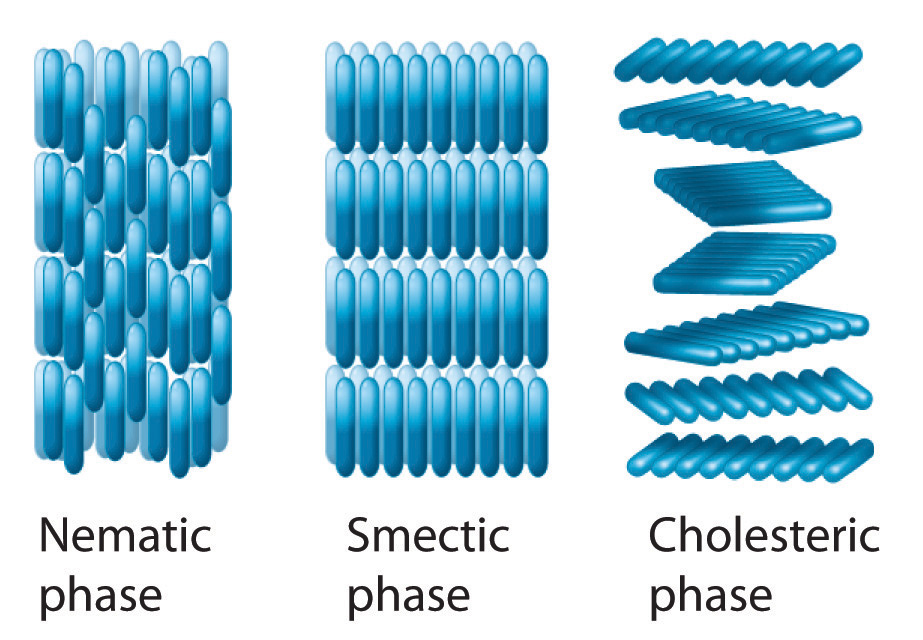
\includegraphics[width=0.6\textwidth]{../lessons/16_image/LC.png}
 \caption{\label{fig:16_LC} Graphical representation of the nematic, smectic and cholesteric phases of a liquid crystal.}
 \end{figure}


\noindent There is a plethora of possible liquid crystal phases; the most common are:

\begin{itemize}
\item \textbf{Nematic}: this phase is characterized by a very strong long-ranged orientational order: the main axes of the molecules tend to orientate along a preferred direction (see Figure \ref{fig:16_9}), determined by the director. There is no long-ranged translational order of the molecular centers of mass, even if a short-ranged one can exist.

From optical point of view the Nematic phase is birifrangent, i.e. they exhibit two different refractive indexes: one parallel to the director \( \overset{\leftrightarrow}{n}  \) (called ordinary refractive index) and one orthogonal to it (special refractive index). These optical properties of the nematic phase are used to build devices like LCDs.

\item \textbf{Smectic}: also in this phase the molecules are aligned along a preferred direction, but contrarily to the nematic one this phase has also a spatial periodic order: the molecules are organised in layers. Furthermore, differently from nematic phases, smectic liquid crystals have non-uniform density and are generally more viscous.

\item \textbf{Cholesteric}: It is similar to the nematic phase since it has a long-ranged orientational order, but the direction of \( \overset{\leftrightarrow}{n}\) changes regularly in space; the typical configuration of a cholesteric liquid crystal has a director \( \overset{\leftrightarrow}{n} (\va{r}) \) that rotates when  \( \va{r} \)  varies along a particular direction: for example, in a three-dimensional reference frame the molecules are orientated along the \( y \)  direction in \( xy \)  plane, but this direction roteates if \( z \) changes.

The structure of a cholesteric liquid crystal is characterised by the spatial distance along the torsion axis, called pitch, after which the director has rotated by an angle of \( 2 \pi  \). The pitch of the most common cholesteric liquid crystals is of the order of several hundred nanometers, so comparable with the wavelength of visible light; furthermore, it can also be very sensitive to changes in temperature, chemical composition, or external electromagnetic fields. Note also that a nematic liquid crystal can be seen as a cholesteric one with infinite pitch; these two phases in fact are not independent from each other, and there is no real phase transition between them.

\end{itemize}

\begin{figure}[h!]
\begin{minipage}[c]{0.5\linewidth}
\subfloat[][Isotropic phase.]{ 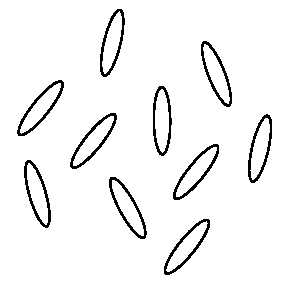
\includegraphics[width=0.8\textwidth]{../lessons/16_image/9.pdf}  \label{fig:16_9_1} }
\end{minipage}
\begin{minipage}[]{0.5\linewidth}
\centering
\subfloat[][Nematic phase.]{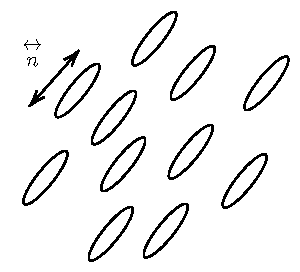
\includegraphics[width=0.8\textwidth]{../lessons/16_image/10.pdf}  \label{fig:16_9_2} }
\end{minipage}
\caption{\label{fig:16_9} }
\end{figure}



\subsection{Definition of an order parameter for nematic liquid crystals}
What we now want to do is to apply Landau theory to liquid crystals in order to study the transition from an isotropic to a nematic phase (Figure \ref{fig:16_9}); therefore, we must define an order parameter for such a system. This is absolutely not trivial, and there are two ways to do it a microscopic and a macroscopic one. We will use a macroscopic approach.

\subsubsection{Macroscopic approach}
From a macroscopic point of view we have already stated that an important difference between the disordered and nematic phases consists in the response functions when the liquid crystal is subjected to magnetic or electrical fields. Hence, a macroscopic definition of an order parameter for LC phase is based on the system response when subject to fields. For instance, supposing that we have a liquid crystal subject to an external magnetic field \( \va{H} \), the diamagnetic response of the system will be measurable in terms of its magnetization \( \va{M} \), and in particular:
\begin{equation}
  \va{M} = \bar{\bar{\chi } } \va{H}
\end{equation}
where  \(  \bar{\bar{\chi } } \) is the response function matrix, namely the magnetic susceptibility of the system. In components we have:
\begin{equation}
  M_ \alpha = \chi _{\alpha \beta } H _{\beta }
\end{equation}
where the inexes \( \alpha , \beta  \) stands for \( x,y,z \). If \( \va{H} \) is static, then \( \chi  \) is symmetric, i.e.
\begin{equation*}
  \chi _{\alpha \beta } = \chi _{\beta \alpha }
\end{equation*}
In the isotropic phase \( \chi  \) will also be diagonal, namely
\begin{equation*}
  \chi _{\alpha \beta } = \chi  \delta _{\alpha \beta }
\end{equation*}
while in the nematic phase
For a LC in the neumatic one has
\begin{equation}
  \chi _{\alpha \beta } =
  \begin{pmatrix}
  \chi _\bot   &  0 & 0 \\
    0 &  \chi _ \bot & 0 \\
    0 &  0 &  \chi _\parallel
  \end{pmatrix}
\end{equation}
where, as before, we have supposed that the director \( \overset{\leftrightarrow}{n} \) is parallel to the \( z \) direction.

Therefore we could build an order parameter in terms of the susceptibility \( \chi  \), and this parameter will necessarily have a tensorial nature (since \( \chi  \) itself is in general a tensor), so it will not be a simple scalar like in the previous case. Since we want our order parameter to vanish in the disordered phase, we can define it "removing" from \( \chi  \) its isotropic component. In other words, in components we can define:
\begin{equation}
  Q_{\alpha \beta } = A \qty(\chi _{\alpha \beta } - \frac{1}{3} \delta _{\alpha \beta }\Tr \bar{\bar{\chi } }  )
\end{equation}
where \( A \) is a constant. In this way \( Q \) is a good tensorial order parameter. In particular, the order parameter is a second rank traceless tensor. Let us note that its definition is completely general, and in fact it is useful also to describe other kinds of phases, not only the uniaxial nematic one.

 It is possible to show that \(   Q_{\alpha \beta }  \) can be written in terms of the local average orientiational order of the elementary constituents, \(  \overset{\leftrightarrow}{n} (\va{r}) \) and the degree of local order given by a scalar \( S(\va{r}) \). Hence, we can define
\begin{equation}
  Q_{\alpha \beta } (\va{r}) = S (\va{r}) \qty(n_{\alpha } (\va{r}) n_{\beta } (\va{r}) - \frac{1}{3}\delta _{\alpha \beta })
\end{equation}
The advantage of this definition of the order parameter (which is the one we will use in the following) is that it also takes into account the degree of orientation and the mean direction.
By definition \( Q \) is symmetric and traceless\footnote{A matrix whose trace is zero is said to be traceless.}, so in general way we can write it as:
\begin{equation}
  Q  =
  \begin{pmatrix}
  q_1   & q_2  & q_3 \\
  q_2   & q_4  & q_5 \\
  q_3   & q_5  & -q_1-q_4
  \end{pmatrix}
\end{equation}



\subsection{Landau-de Gennes theory for nematic liquid crystals}
Since we now have a proper order parameter, we can formulate the Landau theory for the phase transitions of nematic liquid crystals (also called Landau-de Gennes theory). In particular we want to study the transition between the isotropic and nematic phase, and we call \( T_{n-i} \) the temperature at which it occurs.

As we have already stated, the Landau free energy \( \mathcal{L} \)  must be consistent with the symmetries of the system, so in this case it must be invariant under rotations. Now, since \( Q \) transforms as a tensor under rotations and \( \mathcal{L} \) must be a scalar, it will contain terms of the form  \( \Tr \bar{\bar{Q} }^P \); to the fourth order we will have (the linear term is absent because by definition \( Q \) is traceless, i.e. \( \Tr(Q) = 0  \)):
\begin{equation*}
  \mathcal{L} = \mathcal{L}_0 + \frac{1}{2} A(T) \Tr \bar{\bar{Q} }^2 + \frac{1}{3} B(T) \Tr \bar{\bar{Q} }^3 + \frac{1}{4} C(T) \qty[ \qty(\Tr \bar{\bar{Q} }^2  )^2 + \Tr \bar{\bar{Q} }^4 ]
\end{equation*}

In reality this expression, and in particular the quartic term, can be simplified: in fact it is a property (which we will not prove) of any \( n \times n \)  symmetric matrix that \( \Tr \bar{\bar{Q} }^s \) with \( s>n \)  can be expressed as a
 polynomial of \( \Tr \bar{\bar{Q} }^p \) with \( p<n \), so in our case any \( \Tr \bar{\bar{Q} }^s \) with \( s\geq 4 \) can be expressed in terms of \( \Tr \bar{\bar{Q} }^2 \) and \( \Tr \bar{\bar{Q} }^3 \) (we are automatically neglecting  \( \Tr \bar{\bar{Q} } \)  since in our case it vanishes, but in general it must be considered).
 Therefore, we can write the Landau free energy as:
 \begin{equation}
   \mathcal{L} = \mathcal{L}_0 + \frac{1}{2} A(T) \Tr \bar{\bar{Q} }^2 + \frac{1}{3} B(T) \Tr \bar{\bar{Q} }^3 + \frac{1}{4} C(T)  \qty(\Tr \bar{\bar{Q} }^2  )^2
 \end{equation}
or, in components:
\begin{equation}
  \mathcal{L} = \mathcal{L}_0 + \frac{1}{2} A(T) Q_{\alpha \beta }Q_{\beta \alpha } + \frac{1}{3} B(T) Q_{\alpha \beta } Q_{\beta \gamma  } Q_{\gamma  \alpha }+ \frac{1}{4} C(T) \qty(Q_{\alpha \beta } Q_{\beta  \alpha })^2
\end{equation}

\begin{remark}
Since each \( 3 \times 3 \) matrix satisfies the relation
\begin{equation*}
   \Tr \bar{\bar{Q} }^4 = \frac{1}{2} \qty( \Tr \bar{\bar{Q} }^2)^2
\end{equation*}
the term proportional to \( C(T) \) can be written as \( \frac{1}{2}C(T)  \Tr \bar{\bar{Q} }^4 \).
\end{remark}

Let us note that since our order parameter is a tensor its invariance under rotations does not exclude the possible existence of terms with odd powers of \( Q \) in \( \mathcal{L} \), in particular the cubic one.


For the most general case of a \emph{biaxial}  nematic phase \( \bar{\bar{Q} }  \) can be diagonalized giving
\begin{equation}
  Q_{\alpha \beta } =
  \begin{pmatrix}
  \frac{2}{3}S   & 0  & 0 \\
    0 &  - \frac{1}{3} \qty(S+ \eta  ) & 0 \\
    0 &  0 & - \frac{1}{3}\qty(S- \eta  )
  \end{pmatrix}
\end{equation}
where we remind that \( S \) is the degree of local order.
If \( \eta = 0 \) we have the standard \emph{uniaxial} nematic phase and the order parameter becomes
\begin{equation}
  Q_{\alpha \beta } =
  \begin{pmatrix}
  \frac{2}{3}S   & 0  & 0 \\
    0 &  - \frac{1}{3}S & 0 \\
    0 &  0 & - \frac{1}{3}S
  \end{pmatrix}
  \label{eq:16_4}
\end{equation}

Now, from the expression of \( Q \) in the case of a uniaxial nematic liquid crystal (Eq.\eqref{eq:16_4}) we have:
\begin{equation*}
 \Tr \bar{\bar{Q} }^2  = \frac{2}{3} S^2, \quad \Tr \bar{\bar{Q} }^3  = \frac{2}{9} S^3, \quad \qty(\Tr \bar{\bar{Q} }^2)^2  = \frac{4}{9} S^4
\end{equation*}
Hence, for uniaxial nematic liquid crystal the Landau free energy becomes
\begin{equation}
  \mathcal{L} = \mathcal{L}_0 +  \frac{A(T)} {3}S^2 + \frac{2}{27} B(T) S^3 + \frac{C(T)}{9}  S^4
\end{equation}
so that, supposing that \( B \) and \( C \) do not depend on the temperature (i.e. \( B(T) =B \) and \( C(T) = C \)), while  \( A(T) \simeq A (T-T^*) \), we have:
\begin{equation}
  \mathcal{L} = \mathcal{L}_0 + \frac{A}{3} (T-T^*) S^2 + \frac{2}{27} B S^3 + \frac{C}{9} S^4
\end{equation}
This Landau free energy has exactly the same form of the one we studied in first-order phase transitions in Landau theory (Eq.\eqref{eq:16_5}), with the substitutions:
\begin{equation*}
  a = \frac{2}{3} A, \quad w = -\frac{2}{27} B, \quad b = \frac{4}{9} C
\end{equation*}
Applying the results we have already found  (Eq.\eqref{eq:16_6}), we will have that the first-order transitions between the isotropic and nematic phases occurs at the temperature:
\begin{equation}
  T_{n-i} =  T^* + \frac{4w^2}{ba}=  T^* + \frac{2 B^2}{27 A C}
\end{equation}










\chapter{Role of fluctuations in critical phenomena: Ginzburg criterium, Coarse-graining and Ginzburg-Landau theory of phase}

\section{Importance of fluctuations: the Ginzburg criterium}
Maybe mean field is not a very good approximation in proximity of the critical point. Question: how bad is the mean field approximation in proximity of the critical point?

Mean field approximations neglect the fluctuations of the order parameter in the computation of \( Z \).
This is a rather strong assumption since the correlation length
\begin{equation}
   \xi \overset{T \rightarrow T_c}{\sim } \abs{T-T_c}^{-\nu }
\end{equation}
diverges. Let us estimate the error one does in using the MF approximation.

To fix the ideas let us consider the Ising model. Since
\begin{equation}
  \expval{S_i S_j} \overset{MF}{\longrightarrow } \expval{S_i} \expval{S_j}
\end{equation}
For each pair of spin \( (S_i,S_j) \) the relative error is
\begin{equation}
  E_{ij} = \frac{ \abs{\expval{S_i S_j}  - \expval{S_i} \expval{S_j}}   }{\expval{S_i}\expval{S_j}  }
\end{equation}
We need to compute the correlation function
\begin{equation}
  G_c (i,j) \equiv \expval{S_i S_j} - \expval{S_i} \expval{S_j} = \expval{(S_i -\expval{S_i} )(S_j - \expval{S_j} )}
\end{equation}
Assuming \emph{translational invariance}
\begin{equation}
  G_c (i,j) \rightarrow G_c \qty(\abs{\va{r}_i - \va{r}_j} ) \rightarrow G_c (r)
\end{equation}
\begin{remark}
In order to compute \( G_c (r) \) we cannot assume omogeneity since \( \expval{S_i} = \expval{S_j} = m   \). It implies that \( G_c = 0 \) identically in MF. We have to allow the system to display disomogeneities in space!
\end{remark}

\begin{remark}
If we want to compute the error in the mean field, is always zero. So, if we want calculate the average with respect to fluctuations it does not work. We can either look at the variation in which the field is the internal one, or we can somehow try to make a variation not because of thermal fluctuations but because we control it. We do this by using an external field. This is the response theory with a variation of the field. (lesson)
\end{remark}

Let us discuss an important point. The function \( G_c \) does not only descrive the spatial correlation of the fluctuations but also, through the linear response theory, the way in which \( m \) varies in response to an external non-homogeneous magnetic field. Within a mean field theory this is the  only way to compute \( G_c \)!

Let us see how it works. In order to do that, instead using an \( H \) we use an \( H_i \).

\begin{equation}
  Z [H_i]= \Tr_{\{ S \} } \qty(e^{-\beta \qty(-J \sum_{\expval{ij} }^{} S_i S_j   - \sum_{i}^{} H_i S_i ) } )
\end{equation}
The definition of the thermal average is
\begin{equation}
  \expval{S_i} = \frac{\Tr_{\{ S \} } \qty(S_i e^{-\beta \qty(-J \sum_{\expval{ij} }^{} S_i S_j   - \sum_{i}^{} H_i S_i ) } ) }{Z[H_i]}
  = \beta ^{-1} \pdv{\ln{Z} }{H_i} = - \pdv{F}{H_i}
\end{equation}
Similarly one can show that
\begin{equation}
  \expval{S_i S_j} = \frac{\beta ^{-1}}{Z} \frac{\partial^2{Z} }{\partial{H_i} \partial{H_j}  } \quad (to \, do)
\end{equation}
Hence,
\begin{equation}
\begin{split}
  G_c (i,j) & = \frac{\beta ^{-2}}{Z}  \frac{\partial^2{Z} }{\partial{H_i} \partial{H_j}  }
  - \qty(\frac{\beta ^{-1}}{Z} \pdv{Z}{H_i} ) \qty(\frac{\beta ^{-1}}{Z} \pdv{Z}{H_j} ) \\
  & = \beta ^{-1} \frac{\partial^2{\ln{Z} } }{\partial{H_i} \partial{H_j}  }
  = - \frac{\partial^2{F(\{ H_i \}  )} }{\partial{H_i} \partial{H_j}  }
\end{split}
\end{equation}
\begin{remark}
  The response in \( i \) due to a variation of \( H \) in \( j \) is
  \begin{equation}
    \pdv{}{H_j} \expval{S_i} = \pdv{}{H_j} \qty[\beta ^{-1} \pdv{\ln{Z} }{H_i} ]  =\pdv{}{H_j} \qty[-\pdv{F}{H_i} ] =  \beta G_c (i,j)
  \end{equation}
\end{remark}

The \emph{generating functions} are:
\begin{itemize}
\item \( Z[H_i] \): generating function of \( G(i,j) \).
\item \( \ln{Z[H_i]} = - \beta F  \): generating function of \( G_c (i,j) \).
\end{itemize}

\begin{remark}
  (lesson)
  \begin{equation}
    \pdv{M}{H_j} = \sum_{i}^{} \pdv{\expval{S_i} }{H_j} = \sum_{i}^{} G_c (i,j)
  \end{equation}
  \begin{equation}
    H_j = H_j (H)
  \end{equation}
  \begin{equation}
    \pdv{M}{H} = \sum_{j}^{} \pdv{M}{H_j} \pdv{H_j}{H}
    =  \beta \sum_{ij}^{} G_c (i,j)
  \end{equation}
  the last one is the susceptibility \( \chi _T \).
   Therefore,
   \begin{equation}
     \chi _T = \beta \sum_{i,j}^{} G_c (i,j)
   \end{equation}
   \begin{equation}
     G_c (i,j) \rightarrow G_c (\abs{i-j} ) \sim G (\abs{\va{r}} )
   \end{equation}
\end{remark}
\section{Fluctuation-dissipation relation}
\begin{equation}
  Z_N = \Tr \exp [ \beta J \sum_{\expval{ij} }^{} S_i S_j + H \sum_{i}^{} S_i    ]
\end{equation}
where \( H_i = H\, \forall i \).
\begin{equation}
  M = \sum_{i}^{} \expval{S_i} = \frac{1}{Z} \Tr \sum_{i}^{} S_i    \exp [ \beta J \sum_{\expval{ij} }^{} S_i S_j + H \sum_{i}^{} S_i    ] = \frac{1}{\beta Z_N} \pdv{Z_N}{H}
\end{equation}
Similarly
\begin{equation}
  \sum_{ij}^{} \expval{S_i S_j} \overset{to do}{=} \frac{1}{\beta ^2 Z_n} \pdv[2]{Z_N}{H}
\end{equation}
\begin{equation}
\begin{split}
  \chi _T & = \pdv{m}{H} = \pdv{}{H} \qty[- \frac{1}{N} \pdv{F}{H} ] = \pdv{}{H}  \qty[\frac{1}{N} k_B T \pdv{\ln{Z} }{H} ] \\
  & = \frac{1}{N} k_B T \qty[\pdv[2]{\ln{Z} }{H} ] = \frac{1}{N} k_B T \qty[\frac{1}{Z} \pdv[2]{Z}{H} - \frac{1}{Z^2} \qty(\pdv{Z}{H} )^2 ] \\
  & = \frac{1}{N \beta } \qty[\beta ^2 \sum_{ij}^{} \expval{S_i S_j}  - \beta ^2 \qty(\sum_{i}^{} \expval{S_i}  )^2   ] \\
  & = \frac{\beta }{N} \sum_{ij}^{}  G_c (i,j) = \frac{\beta }{N} \sum_{ij}^{} G_c (\va{r}_i - \va{r}_j) \\
  & = \beta \sum_{i}^{} G_c (\va{x_i})
\end{split}
\end{equation}
where \( \va{x}_i \equiv \va{r}_i - \va{r}_j \).
\begin{equation}
  \Rightarrow \chi _T = (a^d k_B T)^{-1} \int_{\Omega }^{} \dd[d]{\va{r}} G_c (\va{r})
\end{equation}
this is the fluctuation dissipation relation.
\subsection{Computation of \( E_ R  \)}
The total relative error is the \( E_R (r)\) integrated over the region of radius \( R \le \xi  \), i.e. where correlations are not negligible.
\begin{equation}
  E_{TOT} = \frac{\int_{0}^{\xi } G_c (r) \dd[D]{\va{r}}  }{\int_{0}^{\xi }\expval{S_i} \expval{S_j}  \dd[D]{\va{r}} }
\end{equation}
If \( T < T_c \), there is a solution \( \eta (r) = \eta \neq 0 \)
\begin{equation}
  \Rightarrow \expval{S_i} \expval{S_j} \approx \eta ^2
\end{equation}
is uniform in the region \( \abs{\va{r}} < \xi   \).
\begin{equation}
  E_{TOT} \sim \frac{\int_{0}^{\xi } G_c (\va{r}) \dd[D]{\va{r}}  }{\int_{0}^{\xi } \eta ^2 \dd[D]{\va{r}}  } \ll 1
  \label{eq:16_2}
\end{equation}
This is the Ginzburg criterium. If satisfied the mean field theory is a valid approximation.
\subsection{Estimation of \( E_{TOT} \) as \( t \rightarrow 0^- \)  }
The numerator of the \eqref{eq:16_2} can be approximated as
\begin{equation}
  \int_{V_{\xi }}^{} G_c (r)\dd[D]{r} \overset{\substack{ \text{fluctuation} \\  \text{dissipation} } }{\sim } k_B T_c \chi _T \sim t^{-\gamma  }
\end{equation}
On the other hand, the denominator
\begin{equation}
  \int_{V_{\xi }}^{} \eta ^2 \dd[D]{r} \sim \xi ^D \abs{t}^{2 \beta } \sim t^{2 \beta - \nu D}
\end{equation}
To satisfy the Ginzburg criterium
\begin{equation}
  E_{TOT} \overset{t \rightarrow 0^-}{\sim } t^{- \gamma + \nu D - 2 \beta  } \ll 1
\end{equation}
As \( t \rightarrow 0^- \) this is possible only if \( - \gamma + \nu D - 2 \beta >0  \), hence
\begin{empheq}[box=\myyellowbox]{equation}
  D > \frac{\gamma + 2 \beta  }{\nu } \equiv D_c
\end{empheq}
is called the upper critical dimension.
\begin{itemize}
\item For \( D < D_c \): fluctuations are relevant and mean field is no a good approximation.
\item For \( D > D_c \): fluctuations are less important and mean field describes properly the critical point.
\item For \( D = D_c \): mean field critical exponents ok but strong correction to the scaling expected. For a Ising-like systems (in the mean field)
\begin{equation}
  \beta = \frac{1}{2}, \quad \gamma =1 \quad \Rightarrow D_c = \frac{2}{\nu}
\end{equation}
In order to compute \( D_c \) we need to compute \( \nu  \) withing the mean field approximation. We have to consider the system with spatial disomogeneitis!
\begin{remark}
We have \( \nu _{MF} = 1/2 \). Therefore, the dimension is \( D>4 \) for the mean field.
\end{remark}
\end{itemize}
Now we have a lower critical dimension (remember the last lessons!) and an upper one.

















\end{document}
